
%%%%%%%%%%%%%%%%%%%%%%%%%%%%%%%%%%%%%%%%%%%%%%%%%%%%%%%%%%%%%%%
%
% Welcome to Overleaf --- just edit your LaTeX on the left,
% and we'll compile it for you on the right. If you open the
% 'Share' menu, you can invite other users to edit at the same
% time. See www.overleaf.com/learn for more info. Enjoy!
%
%%%%%%%%%%%%%%%%%%%%%%%%%%%%%%%%%%%%%%%%%%%%%%%%%%%%%%%%%%%%%%%
\documentclass{exam}

\usepackage{graphicx}

% \usepackage{physics}
\usepackage{amsmath}
\usepackage{tikz}
\usepackage{mathdots}
% \usepackage{yhmath}
\usepackage{cancel}
\usepackage{color}
% \usepackage{siunitx}
\usepackage{array}
\usepackage{multirow}
\usepackage{amssymb}
\usepackage{gensymb}
\usepackage{tabularx}
% \usepackage{extarrows}
\usepackage{booktabs}
\usetikzlibrary{fadings}
\usetikzlibrary{patterns}
\usetikzlibrary{shadows.blur}
\usetikzlibrary{shapes}


\lhead{ECON 2010}
\chead{Problem Set \#5}
\lfoot{}
\rhead{Fall 2022}

\printanswers
% \noprintanswers

\begin{document}

\section{Graded Questions}

\begin{questions}

\question Sketch the Lorenz curve for a country whose income is distributed as follows:

\begin{center}
\begin{tabular}{l|c}
Quintile & Income Share (\%) \\ \hline
1st & 10 \\
2nd & 15 \\
3rd & 20 \\
4th & 25 \\
5th & 30 \\ \hline
Total Income & \$250,000
\end{tabular}
\end{center}

\begin{parts}
\part If each resident's income increases by 2\%, how will the Lorenz curve change?
\part The government sells oil rights to a foreign mining company and distributes the proceeds equally to each resident. All incomes increase by \$2,000. Is the new Lorenze curve closer or further from the 45-degree line?
\end{parts}

\question Consider the following labor supply graph:




\tikzset{every picture/.style={line width=0.75pt}} %set default line width to 0.75pt        

\centering
\begin{tikzpicture}[x=0.75pt,y=0.75pt,yscale=-1,xscale=1]
%uncomment if require: \path (0,235); %set diagram left start at 0, and has height of 235

%Shape: Axis 2D [id:dp5394672318688845] 
\draw  (90,190.47) -- (300.33,190.47)(111.03,20.67) -- (111.03,209.33) (293.33,185.47) -- (300.33,190.47) -- (293.33,195.47) (106.03,27.67) -- (111.03,20.67) -- (116.03,27.67)  ;
%Curve Lines [id:da007962273771988437] 
\draw    (95,172) .. controls (168.33,164.67) and (277,113.33) .. (182.33,50) ;

% Text Node
\draw (173.33,29) node [anchor=north west][inner sep=0.75pt]   [align=left] {$\displaystyle S$};
% Text Node
\draw (37.3,20.72) node [anchor=north west][inner sep=0.75pt]  [rotate=-359.9] [align=left] {$\displaystyle  \begin{array}{{>{\displaystyle}l}}
\ \ \ wage\\
( \$/hour)
\end{array}$};
% Text Node
\draw (291.33,199) node [anchor=north west][inner sep=0.75pt]   [align=left] {$\displaystyle hours$};
\end{tikzpicture}


\begin{parts}
\part What effect causes the curve to slope upwards?
\part What effect causes it to bend backwards? Explain.
\end{parts}

\raggedright
\pagebreak
\question Consider the market for land on Manhattan. 

\centering




\tikzset{every picture/.style={line width=0.75pt}} %set default line width to 0.75pt        

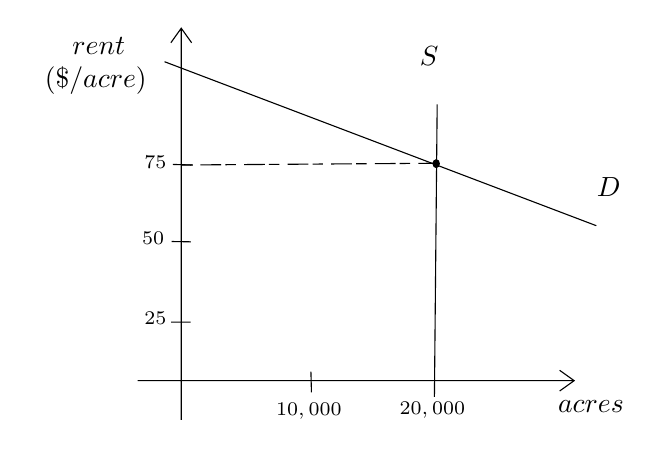
\begin{tikzpicture}[x=0.75pt,y=0.75pt,yscale=-1,xscale=1]
%uncomment if require: \path (0,235); %set diagram left start at 0, and has height of 235

%Shape: Axis 2D [id:dp5394672318688845] 
\draw  (90,190.47) -- (300.33,190.47)(111.03,20.67) -- (111.03,209.33) (293.33,185.47) -- (300.33,190.47) -- (293.33,195.47) (106.03,27.67) -- (111.03,20.67) -- (116.03,27.67)  ;
%Straight Lines [id:da11137620077295463] 
\draw    (234.33,57.33) -- (233,198.25) ;
%Straight Lines [id:da9071355192472479] 
\draw    (103,36.81) -- (311,115.81) ;
%Straight Lines [id:da44969381053897983] 
\draw    (173.5,186.13) -- (173.75,196.13) ;
%Shape: Ellipse [id:dp1468665046840203] 
\draw  [fill={rgb, 255:red, 0; green, 0; blue, 0 }  ,fill opacity=1 ] (232.36,85.91) .. controls (232.36,84.88) and (233.03,84.04) .. (233.86,84.04) .. controls (234.69,84.04) and (235.36,84.88) .. (235.36,85.91) .. controls (235.36,86.95) and (234.69,87.79) .. (233.86,87.79) .. controls (233.03,87.79) and (232.36,86.95) .. (232.36,85.91) -- cycle ;
%Straight Lines [id:da6553318224551603] 
\draw  [dash pattern={on 3.75pt off 3pt on 7.5pt off 1.5pt}]  (111.29,86.57) -- (234.43,85.71) ;
%Straight Lines [id:da8706754814139546] 
\draw    (115.5,162.25) -- (106.14,162.29) ;
%Straight Lines [id:da33632590372576177] 
\draw    (115.67,123.58) -- (106.43,123.43) ;
%Straight Lines [id:da6769961483256663] 
\draw    (116.67,86.58) -- (107,86.29) ;

% Text Node
\draw (224.67,28.33) node [anchor=north west][inner sep=0.75pt]   [align=left] {$\displaystyle S$};
% Text Node
\draw (37.3,20.72) node [anchor=north west][inner sep=0.75pt]  [rotate=-359.9] [align=left] {$\displaystyle  \begin{array}{{>{\displaystyle}l}}
\ \ \ rent\\
( \$/acre)
\end{array}$};
% Text Node
\draw (291.33,199) node [anchor=north west][inner sep=0.75pt]   [align=left] {$\displaystyle acres$};
% Text Node
\draw (310.05,91.48) node [anchor=north west][inner sep=0.75pt]   [align=left] {$\displaystyle D$};
% Text Node
\draw (155.5,200.07) node [anchor=north west][inner sep=0.75pt]  [font=\scriptsize] [align=left] {$\displaystyle 10,000$};
% Text Node
\draw (215,199.5) node [anchor=north west][inner sep=0.75pt]  [font=\scriptsize] [align=left] {$\displaystyle 20,000$};
% Text Node
\draw (91.95,80.98) node [anchor=north west][inner sep=0.75pt]  [font=\scriptsize] [align=left] {$\displaystyle 75$};
% Text Node
\draw (90.95,117.67) node [anchor=north west][inner sep=0.75pt]  [font=\scriptsize] [align=left] {$\displaystyle 50$};
% Text Node
\draw (91.95,156) node [anchor=north west][inner sep=0.75pt]  [font=\scriptsize] [align=left] {$\displaystyle 25$};


\end{tikzpicture}


\raggedright
\begin{parts}
\part Landowners rent their property to commercial and residential tenents. Landlords must pay \$50/acre to maintain their land. What is the economic rent earned by the landlords of Manhattan per acre?
\part Suppose that the city government imposes a \$10/acre tax on land rentals. Who bears the burden of the tax: renters, or land owners?
\part Illustrate the effect of the tax on the graph.
\part In general, why are taxes on economic rents preferable to other taxes?
\end{parts}


\question The Wal-Mart in a rural town is the only major employer. 
\begin{parts}
\part Draw a graph of the labor market under the assumption that Wal-Mart has monopsony power. Include demand, supply, and the marginal factor cost. 
\part Identify the equilibrium wage and quantity.
\part Show how a minimum wage can raise both the wage and the quantity of labor in this market.
\end{parts}

\end{questions}




\end{document}
